%%%%%%%%%%%%%%%%%%%%%%%%%%%%%%%%%% NAME %%%%%%%%%%%%%%%%%%%%%%%%%%%%%

%%%%%%%%%%%%%%%%%
\section{Stability Analysis}

\subsection{Root Locus}
\begin{frame}{Stability Analysis}{Root Locus}
\begin{minipage}{\linewidth}
	\begin{minipage}{0.45\linewidth}
		\begin{figure}
			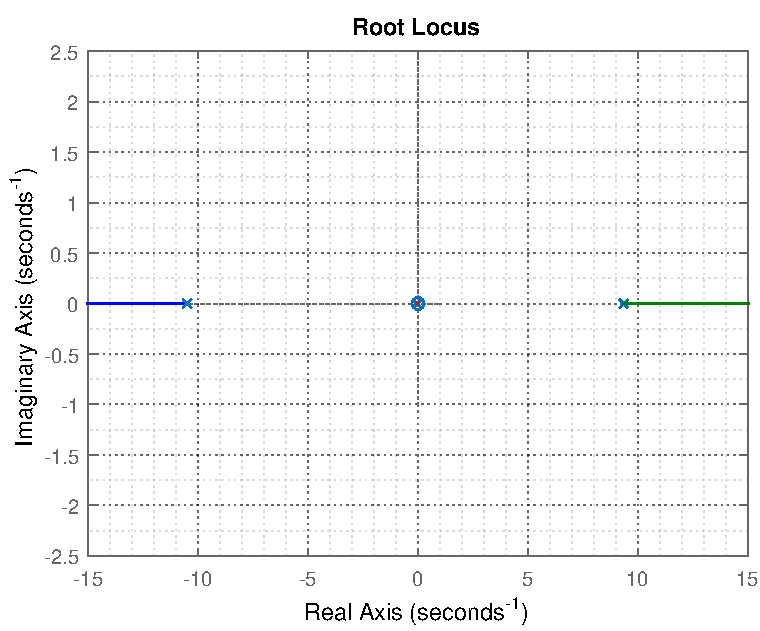
\includegraphics[scale=.42]{Pictures/rlocusCubli}
			\centering
		\end{figure}
	\end{minipage}
	\hspace{0.1\linewidth}
	\begin{minipage}{0.45\linewidth}
		\begin{figure}[H]
			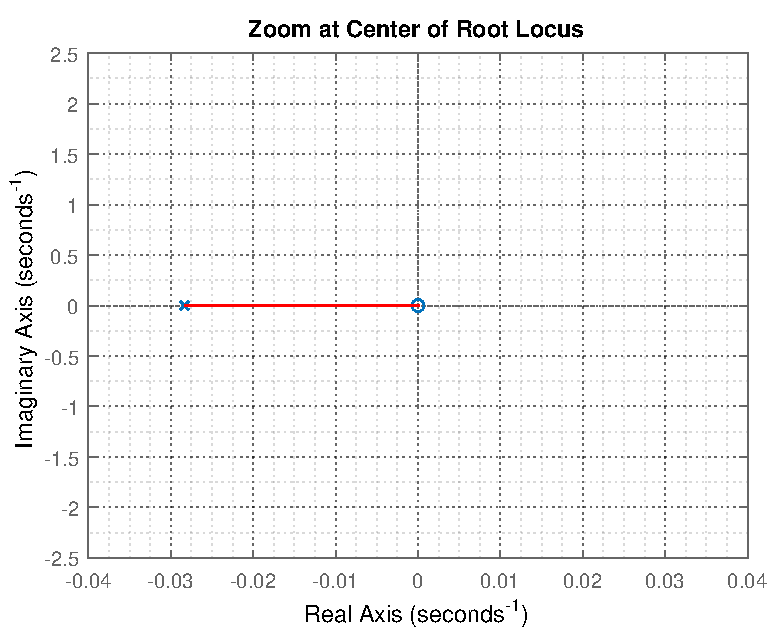
\includegraphics[scale=.35]{Pictures/rlocusCubliZoom}
			\centering
		\end{figure}
	\end{minipage}
\end{minipage}
\end{frame}

\subsection{Nyquist Plot}
\begin{frame}{Stability Analysis}{Nyquist Plot}
\begin{figure}
		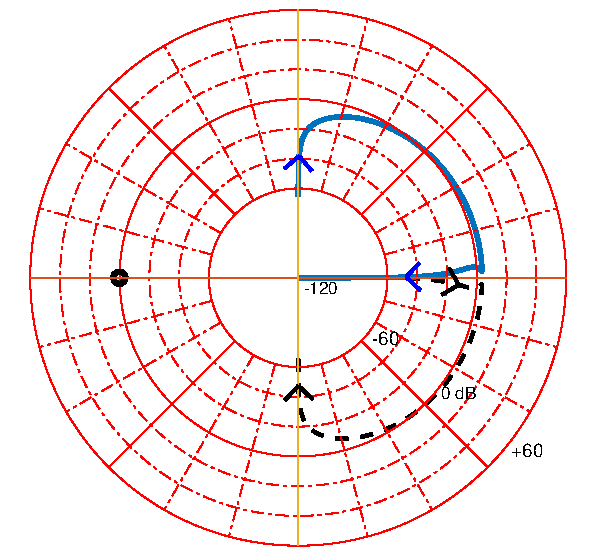
\includegraphics[scale=.5]{Pictures/nyquistCubli}
		\centering
\end{figure}
	
\end{frame}
%%%%%%%%%%%%%%%%%

%%%%%%%%%%%%%%%%%
\section{Classical Controller Design}

\subsection{SISO Block Diagram}
\begin{frame}{Classical Controller Design}{SISO Block Diagram}	
\begin{figure}
	\begin{tikzpicture}[ auto,
thick,                         %<--setting line style
node distance=1.5cm,             %<--setting default node distance
scale=0.75,                     %<--|these two scale the whole thing
every node/.style={scale=0.62}, %<  |(always change both)
>=triangle 45 ]

%-- Blocks creation --%
\draw
% DIRECT TERM %
node[shape=coordinate][](input1) at (0,0){}
node[shape=coordinate][](feed) at (0.5,0){}
node(sum1) at (2,0) [sum] {$\sum$}
node(controller) at (4,0) [block]{\Large $D(s)$}
node(plant) at (6,0) [block]{\Large $G(s)$}
node[shape=coordinate][](DummyNode) at (5,-1.5){}
node[shape=coordinate][](FeedbackNode) at (7.5,0){}
;

%-- Block linking --%
% INPUT %
\draw[-](input1)        -- node{\Large $U(s)$}(feed);
\draw[->](feed)  -- (sum1);

% OUTPUT %
\draw[-](plant)  -- (FeedbackNode);
\draw[->](FeedbackNode)       -- node {\Large $Y(s)$} (9,0);

% DIRECT TERM %
\draw[->] (sum1)            -- (controller);
\draw[->] (controller)       -- (plant);

% FEEDBACKS %
\draw[-] (FeedbackNode)  |- (DummyNode);
\draw[->] (DummyNode)  -| (sum1);

%-- Nodes --%
\draw%--------------------------------------------------------------
node at (input1)            [shift={(-0.04, -0.05 )}] {\Large \textbullet}
node at (FeedbackNode)      [shift={(0, -0.07 )}] {\Large \textbullet}
;
%-- Summation signs --%
\draw%--------------------------------------------------------------
node at (sum1) [right = -6.6mm, below = .6mm] {$+$}
node at (sum1) [right = -3mm, below = 3.9mm]  {$-$}
;

\end{tikzpicture} 
\end{figure}
\vspace{.2cm}

\centering
U(s) refers to the desired angular position of the frame \linebreak
\linebreak
Y(s) refers to the actual angular position of the frame

\end{frame}

\subsection{}
\begin{frame}{Classical Controller Design}{}	
	\begin{figure}
		\begin{tikzpicture}[ auto,
thick,                         %<--setting line style
node distance=1.5cm,             %<--setting default node distance
scale=0.75,                     %<--|these two scale the whole thing
every node/.style={scale=0.62}, %<  |(always change both)
>=triangle 45 ]

%-- Blocks creation --%
\draw
% DIRECT TERM %
node[shape=coordinate][](input1) at (0,0){}
node[shape=coordinate][](feed) at (0.5,0){}
node(sum1) at (2,0) [sum] {$\sum$}
node(controller) at (4,0) [block]{\Large $D(s)$}
node(plant) at (6,0) [block]{\Large $G(s)$}
node[shape=coordinate][](DummyNode) at (5,-1.5){}
node[shape=coordinate][](FeedbackNode) at (7.5,0){}
;

%-- Block linking --%
% INPUT %
\draw[-](input1)        -- node{\Large $U(s)$}(feed);
\draw[->](feed)  -- (sum1);

% OUTPUT %
\draw[-](plant)  -- (FeedbackNode);
\draw[->](FeedbackNode)       -- node {\Large $Y(s)$} (9,0);

% DIRECT TERM %
\draw[->] (sum1)            -- (controller);
\draw[->] (controller)       -- (plant);

% FEEDBACKS %
\draw[-] (FeedbackNode)  |- (DummyNode);
\draw[->] (DummyNode)  -| (sum1);

%-- Nodes --%
\draw%--------------------------------------------------------------
node at (input1)            [shift={(-0.04, -0.05 )}] {\Large \textbullet}
node at (FeedbackNode)      [shift={(0, -0.07 )}] {\Large \textbullet}
;
%-- Summation signs --%
\draw%--------------------------------------------------------------
node at (sum1) [right = -6.6mm, below = .6mm] {$+$}
node at (sum1) [right = -3mm, below = 3.9mm]  {$-$}
;

\end{tikzpicture} 
	\end{figure}
\end{frame}

\subsection{Final Controller}
\begin{frame}{Root Locus Designed Controller}{Final Root Locus}
\begin{figure}
	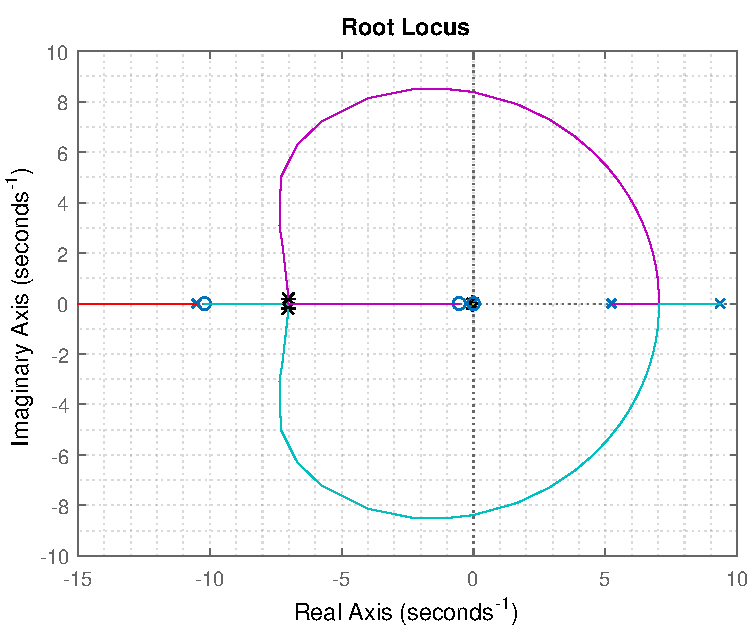
\includegraphics[scale=.435]{Pictures/RLController}
	\centering
\end{figure}	
%
\pause
%
\begin{displaymath}
	D(s)\ =\ -4582,2 \cdot \frac{(s + 9,488)\cdot (s + 1,599)}{(s - 5,54) \cdot (s + 100) \cdot (s + 200)} \nonumber
\end{displaymath}
\end{frame}

\subsection{Discretization}
\begin{frame}{Root Locus Designed Controller}{Discretization}
	
\begin{figure}
	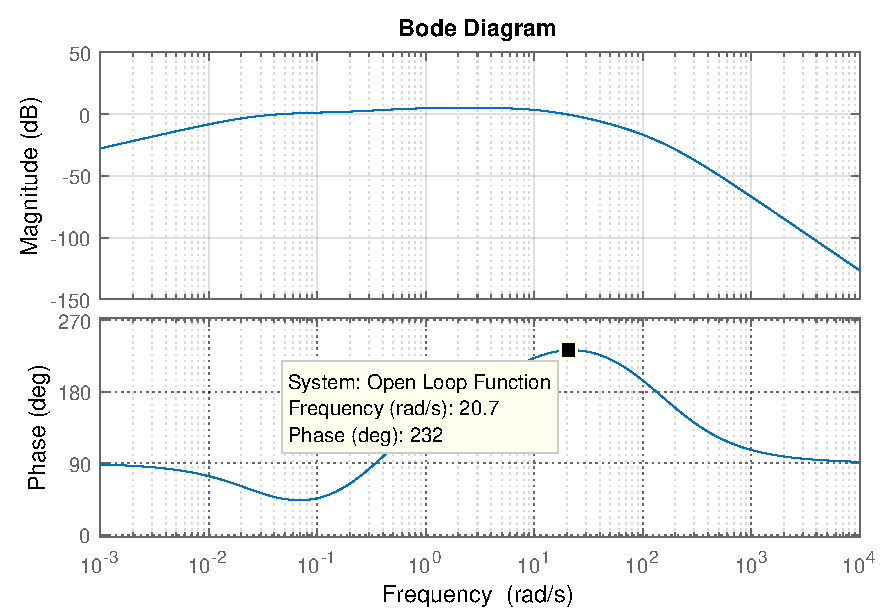
\includegraphics[scale=.435]{Pictures/bodeOL}
\end{figure}
	
\begin{displaymath}
	D(z)\ =\ \frac{\tau_{m,w}(z)}{e_{\theta}(z)}\  = \frac{-8,314 + 7,422 \cdot z^{-1} + 8,302 \cdot z^{-2} - 7,434 \cdot z^{-3}}{1 - 1,382 \cdot z^{-1} + 0,3415 \cdot z^{-2} + 0,001638 \cdot z^{-3}}  \nonumber 
\end{displaymath}
\end{frame}

\begin{frame}{Root Locus Designed Controller}{}	
\begin{figure}
	\begin{tikzpicture}[ auto,
thick,                         %<--setting line style
node distance=1.5cm,             %<--setting default node distance
scale=0.75,                     %<--|these two scale the whole thing
every node/.style={scale=0.62}, %<  |(always change both)
>=triangle 45 ]

%-- Blocks creation --%
\draw
% DIRECT TERM %
node[shape=coordinate][](input1) at (0,0){}
node[shape=coordinate][](feed) at (0.5,0){}
node(sum1) at (2,0) [sum] {$\sum$}
node(controller) at (4,0) [block]{\Large $D(s)$}
node(plant) at (6,0) [block]{\Large $G(s)$}
node[shape=coordinate][](DummyNode) at (5,-1.5){}
node[shape=coordinate][](FeedbackNode) at (7.5,0){}
;

%-- Block linking --%
% INPUT %
\draw[-](input1)        -- node{\Large $U(s)$}(feed);
\draw[->](feed)  -- (sum1);

% OUTPUT %
\draw[-](plant)  -- (FeedbackNode);
\draw[->](FeedbackNode)       -- node {\Large $Y(s)$} (9,0);

% DIRECT TERM %
\draw[->] (sum1)            -- (controller);
\draw[->] (controller)       -- (plant);

% FEEDBACKS %
\draw[-] (FeedbackNode)  |- (DummyNode);
\draw[->] (DummyNode)  -| (sum1);

%-- Nodes --%
\draw%--------------------------------------------------------------
node at (input1)            [shift={(-0.04, -0.05 )}] {\Large \textbullet}
node at (FeedbackNode)      [shift={(0, -0.07 )}] {\Large \textbullet}
;
%-- Summation signs --%
\draw%--------------------------------------------------------------
node at (sum1) [right = -6.6mm, below = .6mm] {$+$}
node at (sum1) [right = -3mm, below = 3.9mm]  {$-$}
;

\end{tikzpicture} 
\end{figure}
\end{frame}
%%%%%%%%%%%%%%%%%
